\documentclass[10pt,conference]{IEEEtran}
\IEEEoverridecommandlockouts
%\IEEEpubid{\makebox[\columnwidth]{978-1-5386-9242-4/18/\$31.00~\copyright2018
%IEEE\hfill}\hspace{\columnsep}\makebox[\columnwidth]{}} 
% The preceding line is only needed to identify funding in the first footnote. If that is unneeded, please comment it out.
\usepackage{cite}
\usepackage{amsmath,amssymb,amsfonts}
\usepackage{algorithmic}
\usepackage{graphicx}
\usepackage{textcomp}
\usepackage{xcolor}
\def\BibTeX{{\rm B\kern-.05em{\sc i\kern-.025em b}\kern-.08em
    T\kern-.1667em\lower.7ex\hbox{E}\kern-.125emX}}
\ifCLASSOPTIONcompsoc
\usepackage[caption=false,font=normalsize,labelfon
t=sf,textfont=sf]{subfig}
\else
\usepackage[caption=false,font=footnotesize]{subfi
g}
\fi
\usepackage{sistyle}    %SI unit style
\usepackage{romannum}   %Roman numbering style
\usepackage{gensymb}    %math symbol
\usepackage{url}        %URL
%====================================

\makeatletter

% title page
\def\ps@IEEEtitlepagestyle{%
\def\@oddhead{\parbox[t][\height][t]{\textwidth}{\raggedleft
2018 21st International Conference of Computer and Information Technology (ICCIT),\\
21-23 December, 2018\\
\noindent\makebox[\linewidth]{\rule{\textwidth}{0.4pt}}
}\hfil\hbox{}}%

\def\@oddfoot{978-1-5386-9242-4/18/\$31.00~\copyright2018
IEEE \hfil 
\leftmark\mbox{}}%
}

\makeatother
% make changes take effect
\pagestyle{headings}
% adjust as needed
\addtolength{\footskip}{0\baselineskip}
\addtolength{\textheight}{0\baselineskip} 

%====================================
\begin{document}

\title{SALSA is an ICT based educational tool for Astrophysics students to study structure and dynamics of Milky Way Galaxy\\
{\footnotesize}
\thanks{Chalmers University of Technology, Onsala, Sweden.}
}

\author{\IEEEauthorblockN{1\textsuperscript{st} Mir Sakhawat Hossain}
\IEEEauthorblockA{\textit{Department of Mathematics} \\
\textit{Kabi Nazrul Government College}\\
Dhaka, Bangladesh \\
s.hossain18@gmail.com}
\and
\IEEEauthorblockN{2\textsuperscript{nd} Banrupa Mallik}
\IEEEauthorblockA{\textit{Department of Physics} \\
\textit{Begum Badrunnessa Govt. Girls College}\\
Dhaka, Bangladesh \\
banrupamallik@gmail.com}
}

\maketitle

\begin{abstract}
After the discovery of radiation from Galactic Hydrogen gas clouds in 1951, the 21cm wavelength HI line had become the best marker to study spectral profiles in radio astronomy. It has been utilized as an important tracer for the distribution and velocity of molecular gas clouds in the Interstellar that has helped enormously in the understanding of galactic structure. ICT based astronomy and astrophyscis tools have been developed for decades for undergraduate level use including radio telescopes controllable over the Internet at minimal cost. These radio telescopes can effectively be used to study galactic structure and dynamics. This paper presents an observation to study galaxy dynamics and map its spiral structure which was carried out between galactic coordinate longitudes $6\degree$ to $225\degree$ and latitudes $0\degree$ to $35\degree$ with two low cost $2.3$ meters Haystack model type radio frequency receiving systems called SALSA radio telescopes at Onsala Space Observatory in Sweden which is maintained by Chalmers University of Technology. Components of the velocity of Hydrogen gas clouds were calculated using different galactic longitudes and latitudes as a function of galactic distance from the center to plot spiral galactic arms and rotation curves. This radio observational experiment was done by remote operation over the Internet in frequency switching mode. Our project aims to prove the quality and importance of this type of ICT based tools for astronomical education and citizen science.
\end{abstract}

\begin{IEEEkeywords}
Open Educational Resources, STEM, Educational technology, Physics education, Student experiments
\end{IEEEkeywords}

\section{Introduction}
Neutral Hydrogen(HI) at the ground state level is an abundant and uniformly distributed element throughout the interstellar medium(ISM). It is the most ubiquitous element in interstellar  low-density regions but can be detected in $\lambda\approx21$ cm or $\approx1420$ MHz where $\textnormal{H}_2$ is symmetric but not detectable at the radio frequencies\cite{HI2016}. In 1933, Karl Guthe Jansky detected first extraterrestrial radio frequency\cite{jansky1933radio}. In 1945 then Van de Hulst predicted $21$ cm wavelength emission\cite{CJBakker1945}. The same frequency line is also detected by Muller and Oort\cite{muller1951observation} in the same year. A preliminary survey was made by Christiansen and Hindman\cite{christiansen1952preliminary} in Australia. They made this survey with a $7.5$\textnormal{-m} paraboloid and movable radio antenna that had a beam width between half power with direction of $1.9\degree$ horizontally and $2.7\degree$ vertically and it covered galactic longitudes $-10\degree$ to $+10\degree$ in the galactic plane. In Netherlands, Muller and Westerhout\cite{Muller1957} took an extended neutral HI line profile survey and made a catalog approximately in galactic latitude $\pm20\degree$ and longitude $318\degree$ to $220\degree$. Within these periods angular resolution has been developed from $30\degree$ to $30$\,-$\mu$as\cite{kellermann2001development,Middelberg2008}. Recently all-sky mapping in HI line based on EBHIS and GASS has been completed\cite{bekhti2016hi4pi} with angular resolution $16.2\arcsec$ and sensitivity $\sigma_{rms}=43$\,mK. Santo and Ashraf carried out a galactic survey to map the Milky Way galaxy in galactic longitudes $0\degree$ to $225\degree$ in the galactic plane\cite{santo2013mapping} using SALSA radio telescope which was built for EU HOU project\cite{Doran2007}. Considering this observation we have accomplished our observation using the SALSA radio telescope in extended galactic coordinates i.e., galactic longitudes $6\degree$ to $225\degree$ and latitudes $0\degree$ to $35\degree$. We have discussed here SALSA Radio Telescope, Basic block diagram of a SALSA type telescope, galactic geometry for observable parameters, observation details, data analysis and results with plotting and importance of this project.

\section{SALSA Radio Telescope}

\subsection{Basic Details of SALSA}

SALSA is a part of the European Hands-On Universe project(EU-HOU)\cite{Ferlet2006} designed to bring interactive lessons of astronomy to the classroom\cite{SALSAS2018}. There are two SALSA telescopes with the same specification see Table~\ref{Tab:salsa_specification}\cite{ThomasBensby2017}. Anyone can control these telescopes using Internet browser by log in \url{https://vale.oso.chalmers.se/salsa/} for free at any time. 


\begin{table*}[htbp]
\caption{Specification of SALSA}
\begin{center}
\begin{tabular}{|c|c|}
\hline
\textbf{Parameter}&\multicolumn{1}{|c|}{\textbf{Value}} \\
\cline{1-2} 
\hline
Diameter & 2.3 m\\
\hline
Focal length & 0.9 m (f/0.37)\\
\hline
Angular resolution & 7 degree at 1420 MHz\\
\hline
Frequency range & 1420 $\pm$ 20 MHz\\
\hline
Frequency resolution & 9.375 kHz (2.4 MHz over 256 frequency channels )\\
\hline
Noise diode temperature & $\approx$ 100K\\
\hline
System temperature & $\approx$ 500K\\
\hline
Aperture efficiency & $\approx$ 50$\%$\\
\hline
Mount & two-axis azimuth/elevation\\
\hline
Pointing accuracy & $\approx$ 0.2 degree\\
\hline
Travel limits &  0-90$\degree$ vertically, 0-360$\degree$ horizontally\\
\hline
\end{tabular}
\label{Tab:salsa_specification}
\end{center}
\end{table*}

The telescope is composed of several main components:
\begin{itemize}
\item A 2.3 meter satellite dish on a fully steerable, motorized azimuth-elevation mount
\item A rotor controller to run the motors which steer the telescope
\item A feed composed of a helical antenna backed by a cavity
\item A super-heterodyne receiver providing 10 MHz bandwidth centered on the 1420.4 MHz (21-cm) hydrogen line
\item A low-noise amplifier
\item A/D conversion on a dedicated PCI card
\item Software on a desktop computer to receive and process data from the telescope and control it
\end{itemize}

This components are the same as Haystack small radio telescope\cite{DustinJohnson2012}.

\IEEEpubidadjcol

\subsection{Basic Diagram of a Small Radio Telescope}

The SALSA block diagram is the same as the Haystack model see Figure~\ref{fig:block_figure} shows the block diagram of the entire radio system, with fundamental elements, theoretical gain and attenuation of signal for each stage and see Table~\ref{Tab:block_summerize} is a summery of key data of this system\cite{DustinJohnson2012}.

\begin{figure}[htbp]
\centerline{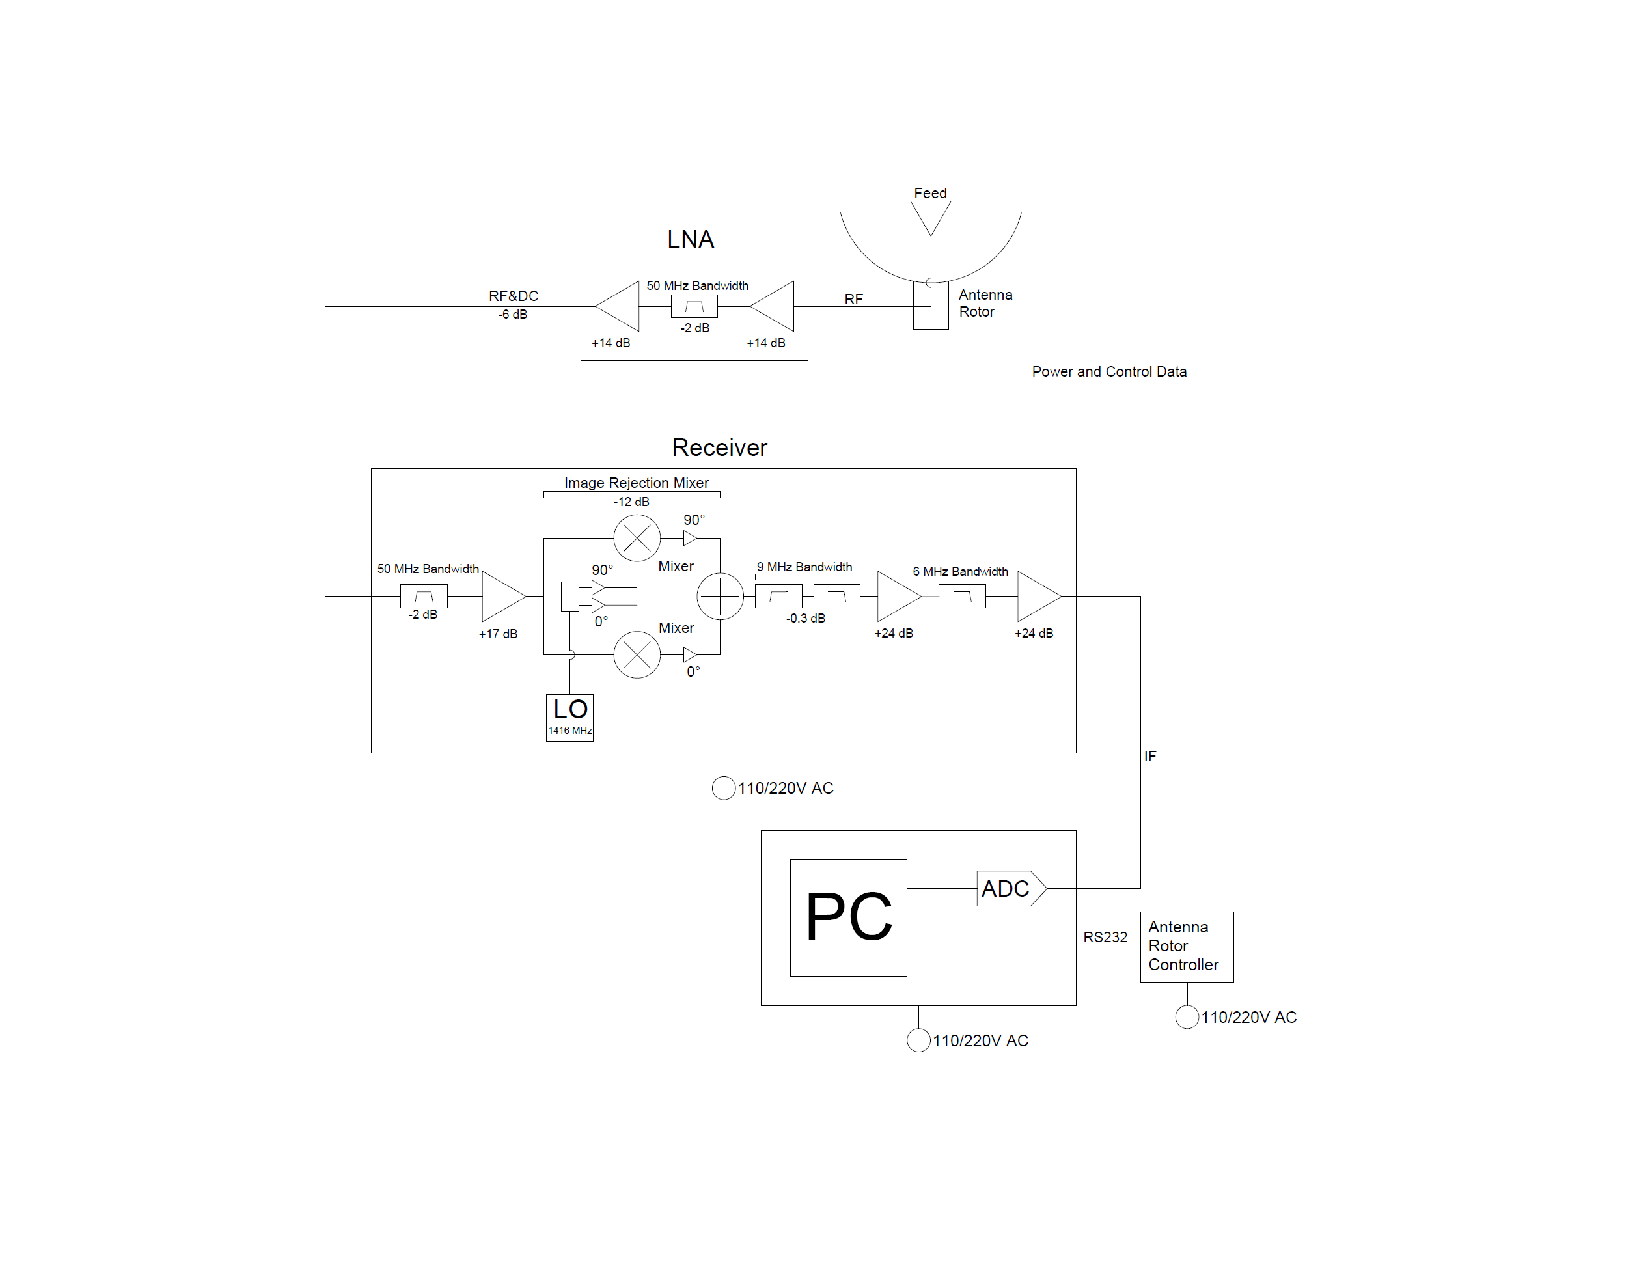
\includegraphics[width=3.5in]{block.pdf}}
\caption{Block Diagram of Haystack Small Radio Telescope}
\label{fig:block_figure}
\end{figure}

\begin{table}[htbp]
\caption{Key data for Haystack small radio telescope}
\begin{center}
\begin{tabular}{|c|c|}
\hline
\textbf{Parameter}&\multicolumn{1}{|c|}{\textbf{Value}} \\
\cline{1-2} 
\hline
Theoretical gain & 71 dB\\
\hline
Measured gain & 71.5 dB\\
\hline
HPBW & 6.5$\degree$\\
\hline
Feed S11 & -23.5 dB\\
\hline
System temperature & 171 K\\
\hline
\end{tabular}
\label{Tab:block_summerize}
\end{center}
\end{table}

\section{Theory}

\subsection{Hyperfine Splitting of Hydrogen}

Neutral Hydrogen consists of a motionless proton(positively charged $+e$) and moving electron(negatively charged $-e$) see Figure~\ref{fig:hyperfine_figure}. The electron orbits around the proton for the mutual attraction of opposite charges. The derivation is as follows Griffiths\cite{griffiths2016introduction}. We can imagine electron is orbiting around nucleus(proton). From the view of an electron, the proton is orbiting electron. This circling creates a magnetic field $\vec{B}$ in the frame of an electron which causes a torque on the spinning electron. It has a tendency to align its magnetic moment($\vec{\mu}$) along the direction of magnetic field\cite{griffiths2016introduction}. So Hamiltonian~(\ref{eq:hamiltonian})

\begin{equation}
  H=-\vec{\mu}\cdot\vec{B}
  \label{eq:hamiltonian} 
\end{equation}

\begin{figure}[htbp]
\centerline{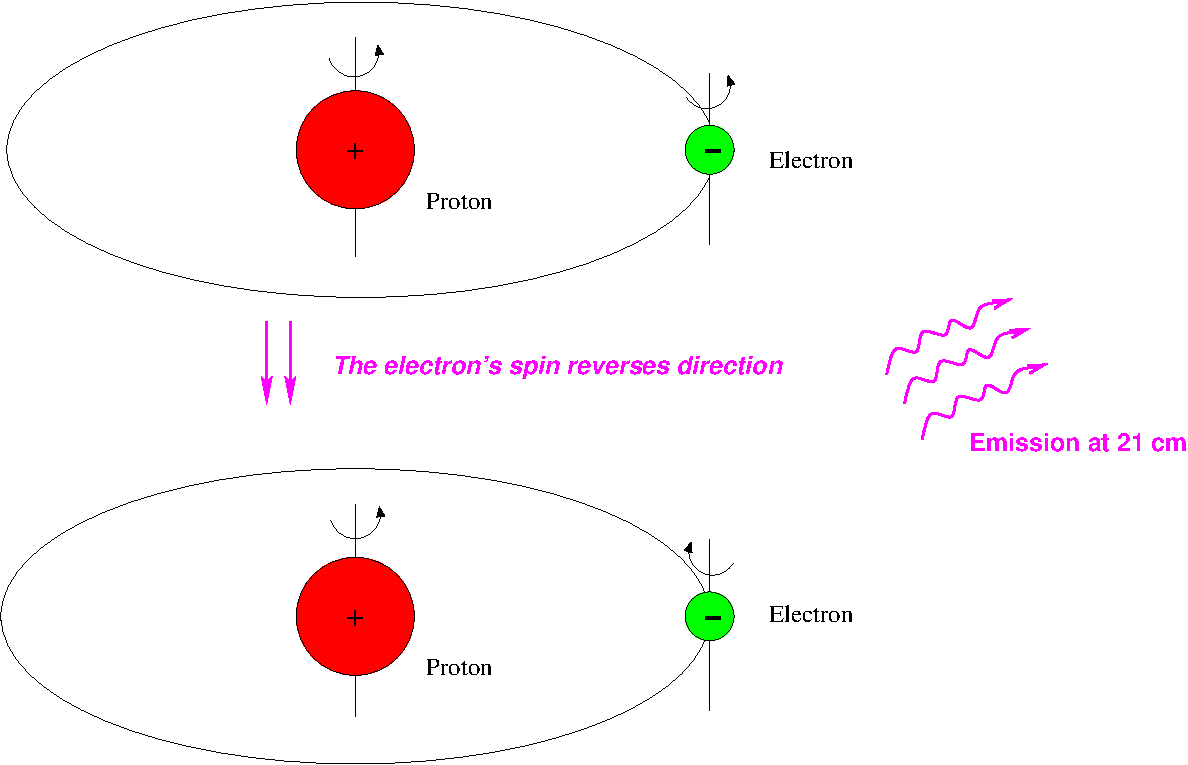
\includegraphics[width=2.5in]{hyperfine.pdf}}
\caption{An illustration of the 21cm transition of the hydrogen atom, caused by the energy change when the electron's spin changes from parallel to the proton's spin to antiparallel\cite{Dante2014}.}
\label{fig:hyperfine_figure}
\end{figure}

We can calculate magnetic field of a proton($\vec{B}$) and dipole moment of an electron($\vec{\mu}$) using Biot Savart law which is~(\ref{eq:biotsavart})

\begin{equation}
  B=\frac{\mu_{0}I}{2r}
  \label{eq:biotsavart}
\end{equation}

Moreover magnetic field $\vec{B}$ and angular momentum $\vec{L}$ are in the same direction, so~(\ref{eq:mag_ang})

\begin{equation}
 \vec{B}=\frac{1}{4\pi\-\epsilon_{0}}\frac{\mathit{e}}{\mathit{mc^{2}r^{3}}}
 \label{eq:mag_ang}
\end{equation}

The direction of magnetic moment $\vec{\mu}$ and spin $\vec{S}$ are the same, so~(\ref{eq:mag_spin})

\begin{equation}
 \vec{\mu}=\frac{\mathit{q}}{2\mathit{m}}\vec{S}
 \label{eq:mag_spin}
\end{equation}

If $\mathit{e}$ is charge of electron, $\mathit{m_{e}}$ is mass of electron and $\vec{S}_{e}$ is spin of electron then magnetic moment of electron is~(\ref{eq:mag_electron}),

\begin{equation}
 \vec{\mu}_{e}=-\frac{\mathit{e}}{\mathit{m_{e}}}\vec{S}_{e}
 \label{eq:mag_electron}
\end{equation}

If $\mathit{m_{e}}$ is mass of proton, ${\vec{S}}_{e}$ is spin of proton and $\vec{g}_{p}$ is g-factor (measured value is 5.59) then magnetic moment of proton is~(\ref{eq:mag_proton}),

\begin{equation}
 \vec{\mu}_{e}=\frac{\mathit{g}_{p}\mathit{e}}{2\mathit{m}_{p}}\vec{S}_{p}
 \label{eq:mag_proton}
\end{equation}

In accordance with classical electrodynamics, the magnetic field produced by dipole $\vec{\mu}$ of the proton sets up magnetic field~(\ref{eq:magfield_proton})

\begin{equation}
 \vec{B}=\frac{\mathit{\mu}_{0}}{4\mathit{\pi}\-\mathit{r}^{3}}[3(\vec{\mu}\cdot\mathit{\hat{r}})\mathit{\hat{r}}-\vec{\mu}]+\frac{2\mathit{\mu}}{3}\vec{\mu}\mathit{\delta}^{3}(\vec{r})
 \label{eq:magfield_proton}
\end{equation}

So Hamiltonian of the electron in the magnetic field due to magnetic dipole moment of proton is~(\ref{eq:dipole_proton})

\begin{equation}
\begin{split}
 \vec{H}'_{hf}=\frac{\mathit{\mu}_{0}g_{p}\mathit{e}^{2}}{8\mathit{\pi}\mathit{m}_{p}\mathit{m}_{e}}\frac{[(3\vec{S}_{e}\cdot\mathit{\hat{r}})(\vec{S}_{e}\cdot\mathit{\hat{r}})]-\vec{S}_{p}\cdot\vec{S}_{e}}{\mathit{r}^{3}}+\\\frac{\mathit{\mu}_{0}g_{p}\mathit{e}^{2}}{3\mathit{m}_{p}\mathit{m}_{e}}\vec{S}_{p}\cdot\vec{S}_{e}\delta^{3}(\vec{r})
\end{split}
 \label{eq:dipole_proton}  
\end{equation}

In accordance with perturbation the first order correction is the expectation value of the perturbing Hamitonian~(\ref{eq:value_hamiltonian})

\begin{equation}
\begin{split}
 \mathit{E}_{hf}^{1}=\frac{\mathit{\mu}_{0}g_{p}\mathit{e}^{2}}{8\mathit{\pi}\mathit{m}_{p}\mathit{m}_{e}}\left\langle\frac{[(3\vec{S}_{e}\cdot\mathit{\hat{r}})(\vec{S}_{e}\cdot\mathit{\hat{r}})]-\vec{S}_{p}\cdot\vec{S}_{e}}{\mathit{r}^{3}}\right\rangle+\\\frac{\mathit{\mu}_{0}g_{p}\mathit{e}^{2}}{3\mathit{m}_{p}\mathit{m}_{e}}\left\langle\vec{S}_{p}\cdot\vec{S}_{e}\right\rangle\vert\mathit{\psi}\left(0\right)\vert^{2}
\end{split}
 \label{eq:value_hamiltonian} 
\end{equation}

In the ground state level, the wave function is spherically symmetrical and the first expectation value vanishes. So we get~(\ref{eq:wave_function})

\begin{equation}
 \mathit{E}_{hf}^{1}=\frac{\mathit{\mu}_{0}g_{p}e^{2}}{3\pi\mathit{m}_{p}\mathit{m}_{e}\mathit{a}^{3}}\left\langle\vec{S}_{p}\cdot\vec{S}_{e}\right\rangle
 \label{eq:wave_function}
\end{equation}

This is called spin-spin coupling because of the dot product of two spin $\vec{S}_{p}$ and $\vec{S}_{e}$. For this coupling the individual spin angular momenta are not conserved. So the good states are eigen vectors of total spin~(\ref{eq:eigen_spin})

\begin{equation}
 \vec{S}\equiv\vec{S}_{e}+\vec{S}_{p}
 \label{eq:eigen_spin}
\end{equation}

By applying total spin states the expected perturbation value can be written as terms of eigen operators as follows~(\ref{eq:spin_perturbation})

\begin{equation}
  \vec{S}_{p}\cdot\vec{S}_{e}=\frac{1}{2}(\mathit{S}^{2}-\mathit{S}_{e}^{2}-\mathit{S}_{p}^{2})
  \label{eq:spin_perturbation}
 \end{equation}
 
But both of electron and proton have spin $1/2$, so\\ $\mathit{S}_{e}^{2}=\mathit{S}_{p}^{2}=(3/4)\mathit{\hbar}^{2}$. In the triplet state(parallel spins) total spin is $1$ and so $\mathit{S}^{2}=2\mathit{\hbar}^{2}$. In the singlet state total spin is $0$ and $\mathit{S}^{2}=0$. Thus~(\ref{eq:total_spin})

\begin{equation}
\label{eq:total_spin}
 \mathit{E}_{hf}^{1}=\frac{4\mathit{g}_{p}\mathit{\hbar}^{4}}{3\mathit{m}_{p}\mathit{m}_{e}^{2}\mathit{c}^{2}\mathit{a}^{4}}\begin{cases}
 +\frac{1}{4}& \text{(triplet)}\\
 -\frac{3}{4}& \text{(singlet)}
\end{cases} 
\end{equation}

The spin-spin coupling breaks the spin degeneracy of the ground state lifting the triplet configuration and depressing the singlet. The energy gap is evidently~(\ref{eq:energy_gap})

\begin{equation}
 \Delta\-E=\frac{4\mathit{g}_{p}\mathit{\hbar}^{4}}{3\mathit{m}_{p}\mathit{m}_{e}^{2}\mathit{c}^{2}\mathit{a}^{4}}=5.88\times10^{-6} eV
 \label{eq:energy_gap}
\end{equation}


The frequency of the photon emitted in a transition from the triplet to the singlet state is~(\ref{eq:singlet_state}),

\begin{equation}
 \mathit{\nu}=\frac{\Delta\-E}{h}=\SI{1420}{MHz}
 \label{eq:singlet_state}
\end{equation}

The corresponding wavelength is $c/\nu=21$ cm which is a part of micro wave region\cite{griffiths2016introduction,santo2013mapping}. In a single Hydrogen atom this transition occurs once per $\approx10^{7}$ years but enormous amount of Hydrogen in spiral arms of Milky Way galaxy causes pervasive and ubiquitous forms of radiation which is observable by radio telescope\cite{santo2013mapping}.

\subsection{Geometry of Galaxy}

The simplified geometry of the Milky Way galaxy\cite{CathyHorellou2015} see Figure.~\ref{fig:galgeo_figure}

\begin{figure}[htbp]
 \includegraphics[width=2.0in]{galgeom}
 \caption{Geometry of the Galaxy. C is the location of the Galactic center, S that of the Sun, M
that of a gas cloud that we want to observe. The SM line is the line-of-sight. The arrow
on an arc indicates the direction of rotation of the Galaxy. The arrows on line segments
indicate the velocity of the Sun ($\vec{V}_0$) and the gas cloud ($\vec{V}$)\cite{CathyHorellou2015}.}
 \label{fig:galgeo_figure}
\end{figure}

There may be a lot of Hydrogen gas clouds in this direction, but for the purpose of this derivation we only care about a single cloud located at position M see Figure.~\ref{fig:galgeo_figure}. Since both the Sun and the cloud are moving, we do not evaluate the cloud velocity directly. Instead, we measure the relative velocity, $\vec{V}_{r}$, between us and the cloud, projected on the line-of-sight\cite{CathyHorellou2015}. Since the observation of Hydrogen gas clouds located at tangential points of galactic plane at different longitudes, the radial velocity of the gas clouds can be written as~(\ref{eq:radial_velocity}),

\begin{equation}
  \vec{V}_{r}=\vec{V}\cos\alpha-\vec{V}_{0}\sin c
  \label{eq:radial_velocity}
\end{equation}

Where $\vec{V}$ is the velocity of gas clouds and $\vec{V}_{0}$ is the velocity of the Sun around galactic center. This equation can be simplified as equation~(\ref{eq:radial_simplified}),

\begin{equation}
 \vec{V}_{r}=\vec{V}\frac{\mathit{R}_{0}}{\mathit{R}}\sin l-\vec{V}_{0}\sin l
 \label{eq:radial_simplified}
\end{equation} 

This equation is for all galactic longitude $\mathit{l}$. Here $\mathit{R}_{0}$ is distance between Sun and galactic center, $\mathit{R}$ is distance between (HI) gas cloud and galactic center. We now assume that gas in Milky Way obeys differential rotation, i.e. the rotational speed is constant with radius and is the same as the rotational speed of the Sun, i.e. equation~(\ref{eq:radial_constant})

\begin{equation}
 \vec{V}_{r}=Constant=\vec{V}_{0}
 \label{eq:radial_constant}
\end{equation}

With this assumption we can write from equation~(\ref{eq:radial_simplified}) we can simplify as a function of cloud distance $\mathit{R}$ and $\vec{V}_{r}$  as follows equation~(\ref{eq:distance_cloud})

\begin{equation}
 \mathit{R}=\frac{\mathit{R}_{0}\vec{V}_{0}\sin l}{\vec{V}_{0}\sin l+\vec{V}_{r}}
 \label{eq:distance_cloud}
\end{equation}

From measurement of radial velocity $\vec{V}_{r}$ we have calculated distance of gas cloud to the galactic centre. With the assumption of $\mathit{R}_{0}=8.5$\,kpc and $\vec{V}_{0}=220$\,km\,s$^{-1}$, we can calculate value of $\mathit{R}$ for different values of galactic longitude $\mathit{l}$. From Figure.~\ref{fig:galgeo_figure} we can see that in the Quadrants \Romannum{1} or \Romannum{4} there can be two possible locations corresponding to given values of $\mathit{l}$ and $\mathit{R}$ to us than the tangential point T (the actual point M on the Figure.~\ref{fig:galgeo_figure}), or farther away, at the intersection of the ST line and the inner circle. But in the Quadrants \Romannum{2} or \Romannum{3} position of the emitting gas clouds can be determined uniquely\cite{CathyHorellou2015}. By the law of cosine in triangle in \textbf{CSM} we have equation~(\ref{eq:cosine_theory}),

\begin{equation}
 \mathit{R}^{2}=\mathit{R}_{0}^{2}+\mathit{r}^{2}-2\mathit{R}_{0}\mathit{r}\cos l
 \label{eq:cosine_theory}
\end{equation}

This is a second-order equation in $\mathit{r}$ where $\mathit{r}$ is distance to cloud from the Sun. The above equation has two possible solutions $\mathit{r}=\mathit{r}_{+}$ and $\mathit{r}=\mathit{r}_{-}$ that can be written as~(\ref{eq:cosine_solution})

\begin{equation}
 \mathit{r}\pm=\pm\sqrt{\mathit{R}^{2}-\mathit{R}_{0}^{2}\sin^{2} l}+\mathit{R}_{0}\cos l
 \label{eq:cosine_solution}
\end{equation}

From equation~(\ref{eq:cosine_solution}) we have discarded negative values and accepted one positive and two positive values. For convenient way of plotting to map the Milky Way structure, we convert the polar coordinate positions given as $\mathit{r}$ and $\mathit{l}$ to Cartesian $\mathbf{x-y}$ coordinates using positive and negative values by~\ref{eqn:rpmtocart}

\begin{equation}
\left\lbrace
\begin{array}{l}
	x=\mathit{r} \cos (\mathit{l}-90\degree) \\
	y=-\mathit{R}_{0}+\mathit{r} \sin (\mathit{l}-90\degree) \\
\end{array}
\right.
\label{eqn:rpmtocart}
\end{equation}

Here we have deducted $\mathit{R}_{0}$ in $\mathbf{y}$ values instead of adding to get image of rotation to fit the Wikipedia image of galactic coordinates and during plotting we converted values from degree to radian. By calculating the value of $\mathbf{x}$ and $\mathbf{y}$ for different velocities at different galactic longitudes $\mathit{l}$ in a graph to plot the map of Milky Way galaxy\cite{CathyHorellou2015,griffiths2016introduction}.

\section{Observations}

This observation was made with SALSA Radio Telescope situated in Onsala Space Observatory, Sweden. This telescope was operated to collect raw data through Internet\footnote{Website address of SALSA web based data collection facility is https://vale.oso.chalmers.se/salsa/welcome} from Dhaka, Bangladesh. There are two radio lab antennas called "Brage" and "Vale". We used both of them. Each antenna has a diameter $2.3$\,-m dish. The angular resolution is $7\degree$ at (HI) radio frequency line($\SI{1420}{MHz}$). Bandwidth of the receivers is $\SI{2.5}{MHz}$ and 256 frequency channels. Width of each channel is $\SI{9.765}{KHz}$. The telescope is controlled by qradio software. The observation was completed in frequency switching mode with reference frequency $\SI{1422.9}{MHz}$ and gain factor $800$\cite{CathyHorellou2015}.

\subsection{Data Reduction}

The observation was made between galactic coordinate longitudes $6\degree$ to $225\degree$ and latitudes $0\degree$ to $35\degree$ following $3\degree$ for galactic longitudes and $5\degree$ for galactic latitudes. The spectra were collected with integration times of $150-300$\,seconds for each. This survey covered $-300<\mathit{V}_{LSR}<300$\,$kms^{-1}$. We tried to collect emission spectrum data at $\mathit{V}_{LSR}\approx 0$\,$kms^{-1}$. By observing radio emission from neutral galactic Hydrogen, we have mapped the motion of Hydrogen gas clouds around the Milky Way galaxy. We have used the Doppler effect to relate observed frequency spectra to the velocity of emitting Hydrogen gas clouds. By the equation of Doppler shift\cite{CathyHorellou2015} we get~(\ref{eq:doppler})

\begin{equation}
 \frac{\mathbf{f}-\mathbf{f}_{0}}{\mathbf{f}_{0}}=-\frac{\vec{v}}{\vec{c}}
 \label{eq:doppler}
\end{equation}

Here $\mathbf{f}$ is the observed frequency, $\mathbf{f}_{0}$ is the rest frequency of line we are observing, $\mathbf{\mathit{v}}$ is the velocity of gas clouds(positive velocity for receding and negative velocity for approaching) and $\vec{c}$ is the velocity of light. Thus we converted frequency spectra to velocity scale then we corrected baselines. After that we applied Gaussian Fit function to smooth the spectra according to the equation~(\ref{eq:gaussianfit})

\begin{equation}
  \mathbf{y}=\sum^n_{i=1}\mathbf{a}_{i}e^{\left[-\left(\frac{\mathbf{x}-\mathbf{b}}{\mathbf{c}_{i}} \right)^{2}\right]}
  \label{eq:gaussianfit}
\end{equation}

Here $\mathbf{a}$ is the amplitude of spectra, $\mathbf{b}$ is the location of the centre of peak, $\mathbf{c}$ is the width of peak and $n$ is the number of peaks to fit\cite{CathyHorellou2015}. We collected peak values with SalsaJ software and SalsaSpectrum\cite{DanielDahlin2015} MATLAB software class file. We have saved all the raw FITS files, Analysis codes, SalsaSpectrum class file and final plotted graphs in a data repository\cite{Hossain2018}.

\subsection{Result}

The Gaussian Fit equation~(\ref{eq:gaussianfit}) has been applied to calculate the central velocity of the spectra. Then we used the equation~(\ref{eq:distance_cloud}) to calculate distance $\mathit{R}$ of the clouds for different longitudes $\mathit{l}$. The values of $\mathit{R}$ has been used to calculate $\mathit{r}$ and checked whether it is single or double positive where we discarded negative values\cite{ThomasBensby2017,santo2013mapping}. We converted these values to the Cartesian coordinates and plotted these coordinates to unravel the spiral structure of Milky Way Galaxy using MATLAB software of version R2017a. Here Perseus arm, Orion arm and other outer arms are clearly identified but some of them are not well recognizable. Here Map of Milky Way in Figure~\ref{fig:map}

\begin{figure*}[!t]
\centering
\subfloat[$\mathit{l}=6\degree-225\degree$ and $\mathit{b}=0\degree$]{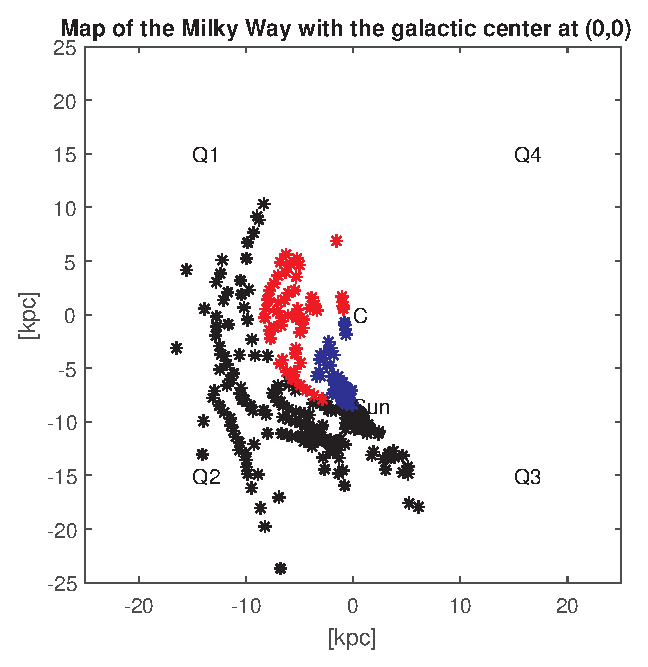
\includegraphics[width=1.5in]{map_1}
\label{fig_first_case}}
\hfil
\subfloat[$\mathit{l}=6\degree-225\degree$ and $\mathit{b}=5\degree$]{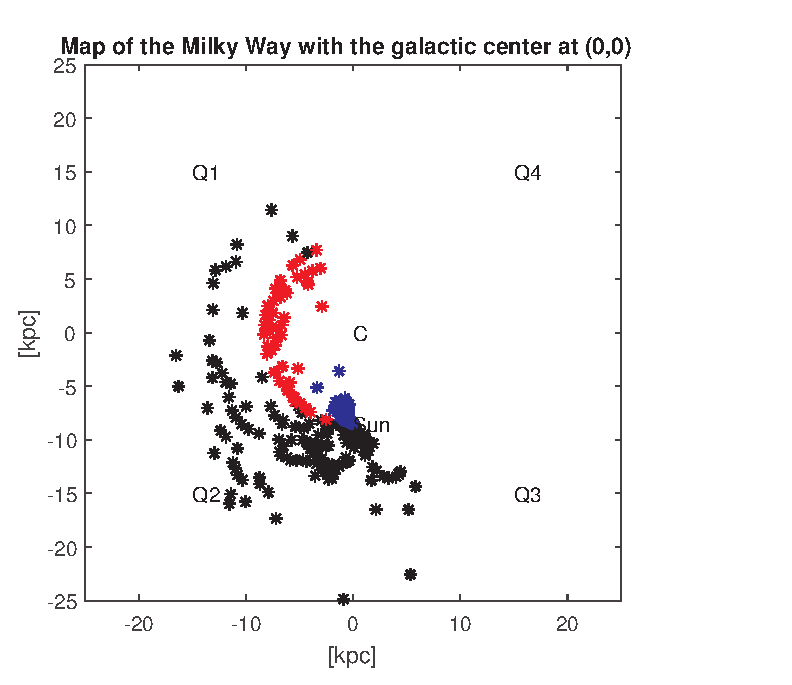
\includegraphics[width=1.5in]{map_2}
\label{fig_second_case}}
\hfil
\subfloat[$\mathit{l}=6\degree-225\degree$ and $\mathit{b}=10\degree$]{\includegraphics[width=1.5in]{map_3}
\label{fig_third_case}}
\hfil
\subfloat[$\mathit{l}=6\degree-225\degree$ and $\mathit{b}=15\degree$]{\includegraphics[width=1.5in]{map_4}
\label{fig_fourth_case}}
\hfil
\subfloat[$\mathit{l}=6\degree-225\degree$ and $\mathit{b}=20\degree$]{\includegraphics[width=1.5in]{map_5}
\label{fig_fifth_case}}
\hfil
\subfloat[$\mathit{l}=6\degree-225\degree$ and $\mathit{b}=25\degree$]{\includegraphics[width=1.5in]{map_6}
\label{fig_sixth_case}}
\hfil
\subfloat[$\mathit{l}=6\degree-225\degree$ and $\mathit{b}=30\degree$]{\includegraphics[width=1.5in]{map_7}
\label{fig_seventh_case}}
\hfil
\subfloat[$\mathit{l}=6\degree-225\degree$ and $\mathit{b}=35\degree$]{\includegraphics[width=1.5in]{map_8}
\label{fig_eighth_case}}
\hfil
\caption{Map of Milky Way at Galactic longitude(l) and Galactic longitude(b)}
\label{fig:map}
\end{figure*}

Moreover we know that rotation curve is a function between circular velocity and radius. By using SALSA Telescope we can calculate the rotation curve of Milky Way\cite{CathyHorellou2015}. We have calculated and plotted the rotation curve see Figure~\ref{fig:rot}. In the data of rotation curve we found that maximum mean $\vec{V(R)}$ is $233.1279$\,$kms^{-1}$($\sigma=120.8813$) and minimum mean $\vec{V(R)}$ is $112.9917$\,$kms^{-1}$($\sigma=73.12281$). Rotation curve of most galaxies which have solar systems shows flat rotation curve i.e. $\vec{V}(\mathit{R})$ does not depend on $\mathit{R}$ beyond certain radius. Angular velocity$\Omega$ varies as $\frac{1}{\mathit{R}}$. Matter near galactic center rotates with a larger angular speed than matter of farther away. But for larger radii this velocity is significantly larger than Keplerian case\cite{CathyHorellou2015}. The figures we have got indication of existence of dark matter see Figure~\ref{fig:rot}

\begin{figure*}[!t]
\centering
\subfloat[$\mathit{l}=6\degree-225\degree$ and $\mathit{b}=0\degree$]{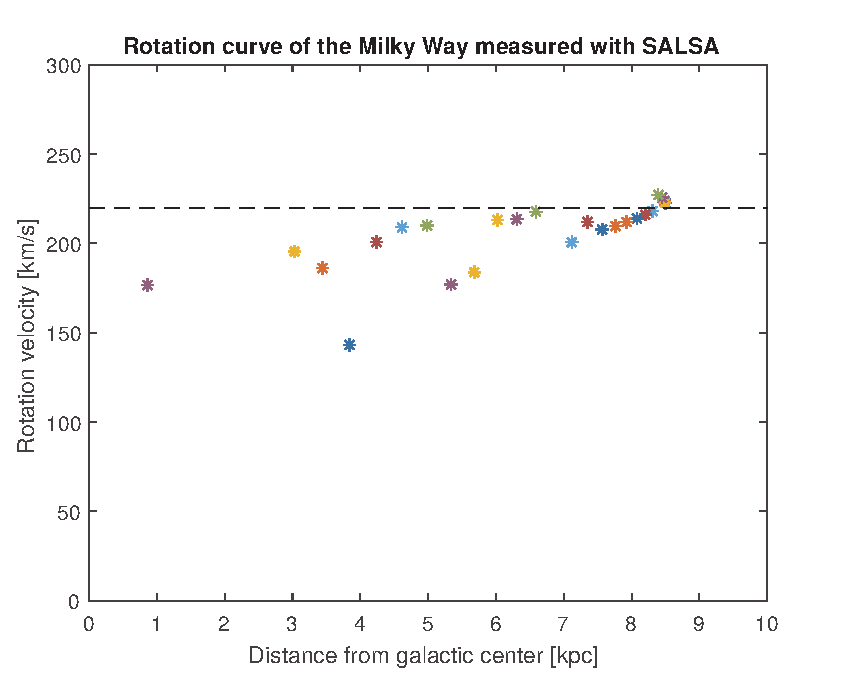
\includegraphics[width=1.5in]{RotationCurve_1}
\label{fig_first_case}}
\hfil
\subfloat[$\mathit{l}=6\degree-225\degree$ and $\mathit{b}=5\degree$]{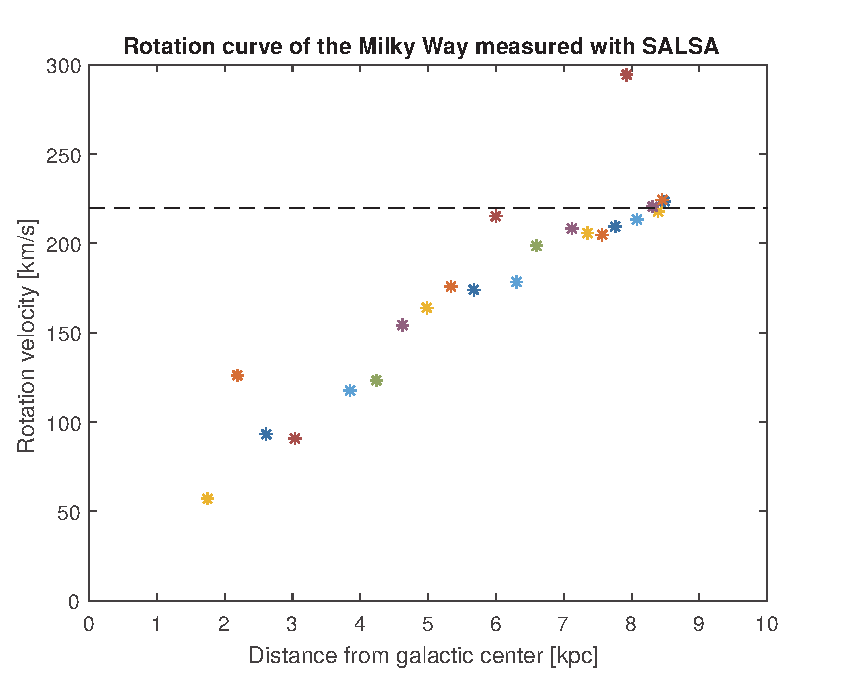
\includegraphics[width=1.5in]{RotationCurve_2}
\label{fig_second_case}}
\hfil
\subfloat[$\mathit{l}=6\degree-225\degree$ and $\mathit{b}=10\degree$]{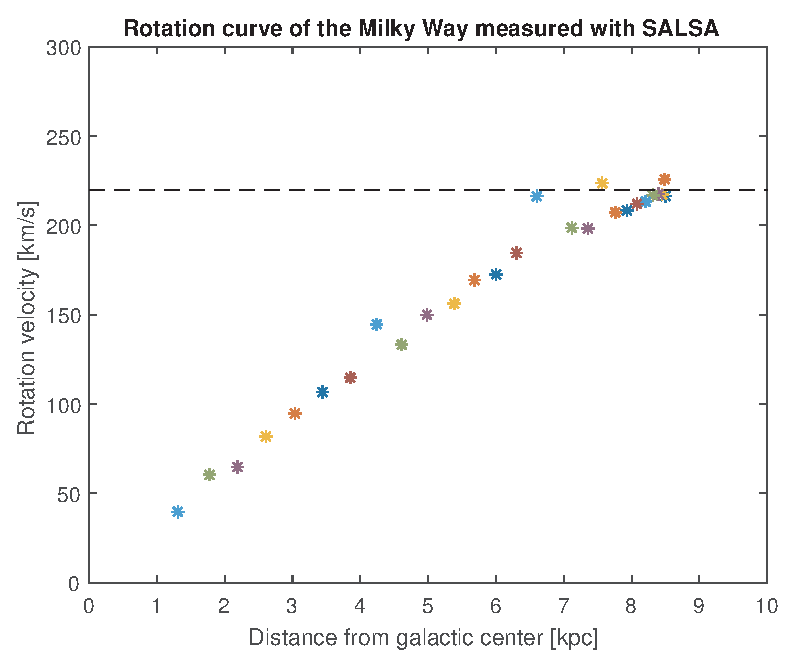
\includegraphics[width=1.5in]{RotationCurve_3}
\label{fig_third_case}}
\hfil
\subfloat[$\mathit{l}=6\degree-225\degree$ and $\mathit{b}=15\degree$]{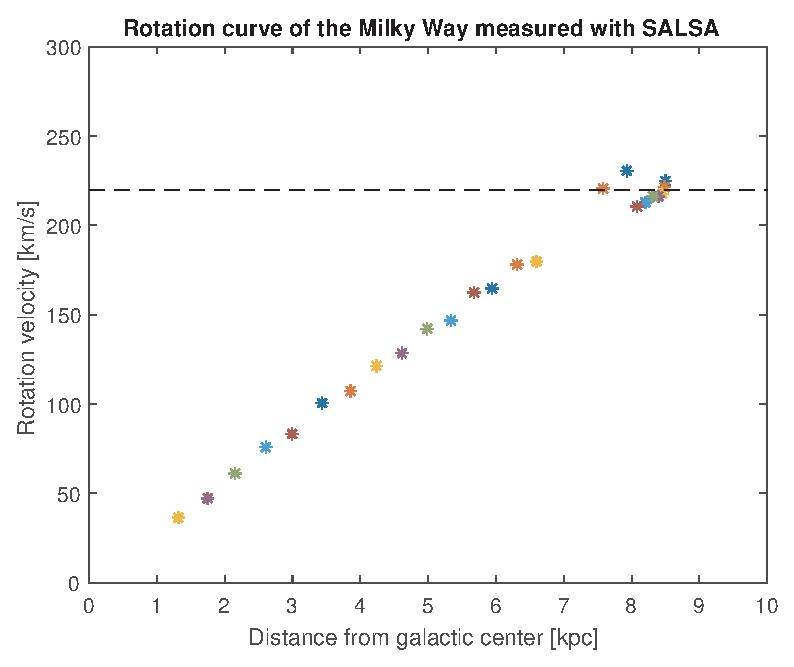
\includegraphics[width=1.5in]{RotationCurve_4}
\label{fig_fourth_case}}
\hfil
\subfloat[$\mathit{l}=6\degree-225\degree$ and $\mathit{b}=20\degree$]{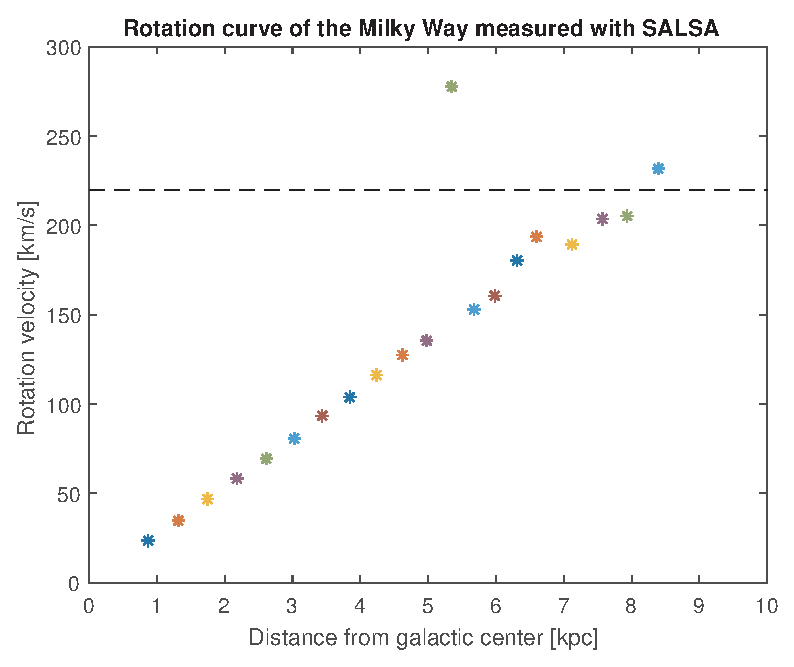
\includegraphics[width=1.5in]{RotationCurve_5}
\label{fig_fifth_case}}
\hfil
\subfloat[$\mathit{l}=6\degree-225\degree$ and $\mathit{b}=25\degree$]{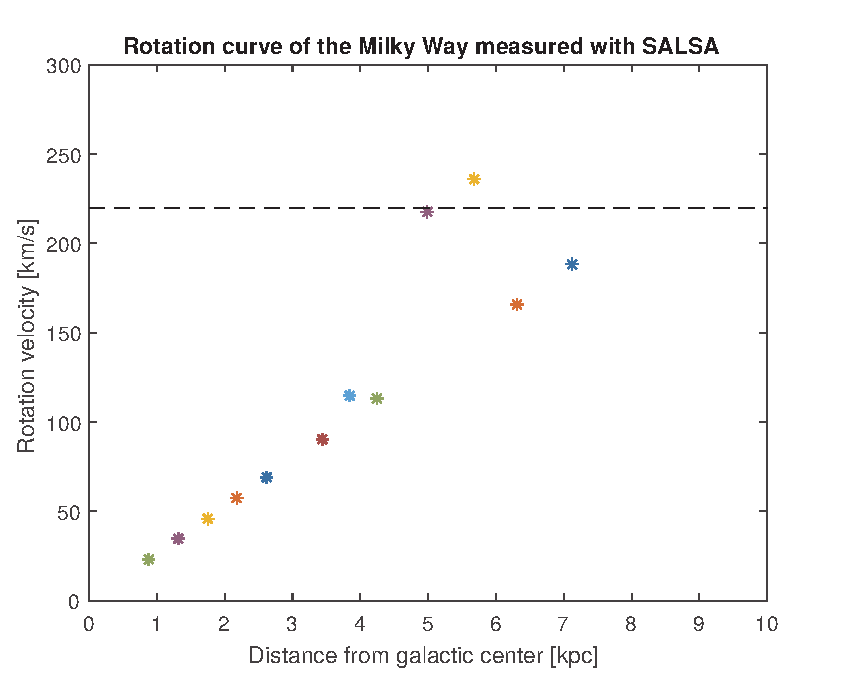
\includegraphics[width=1.5in]{RotationCurve_6}
\label{fig_sixth_case}}
\hfil
\subfloat[$\mathit{l}=6\degree-225\degree$ and $\mathit{b}=30\degree$]{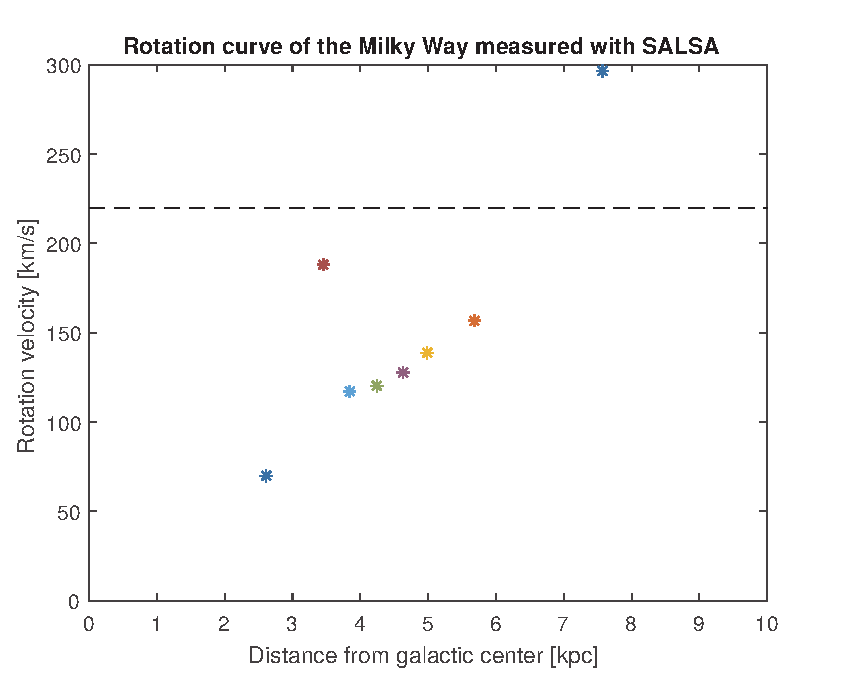
\includegraphics[width=1.5in]{RotationCurve_7}
\label{fig_seventh_case}}
\hfil
\subfloat[$\mathit{l}=6\degree-225\degree$ and $\mathit{b}=35\degree$]{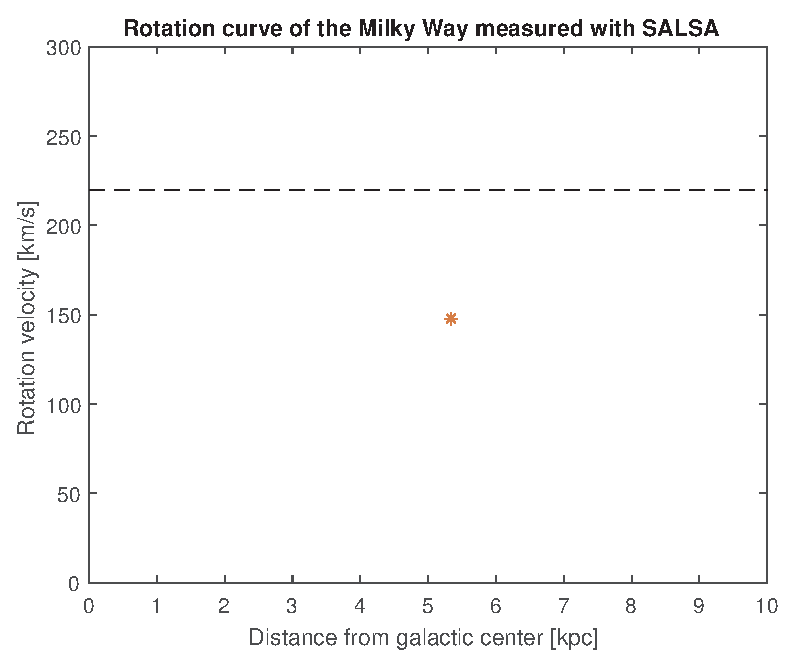
\includegraphics[width=1.5in]{RotationCurve_8}
\label{fig_eighth_case}}
\hfil
\caption{Rotation Curve of Milky Way at Galactic longitude(l) and Galactic longitude(b)}
\label{fig:rot}
\end{figure*}

\section{Limitations and Errors}

The small size of the SALSA telescope limits its sensitivity and resolution. But it has a strong and sensitive receiver and so detected important signals but could not detect the weaker (HI) signals from lower density areas. Below $6\degree$ and above $225\degree$ was not possible to observe for geographical position of telescopes. For this reason we could not observe the whole spiral structure of the Milky Way galaxy. There may be found errors in measuring central velocity of raw spectra\cite{CathyHorellou2015,santo2013mapping}.


\section{Importance of this Experiment}
The aim of this experiment is to describe how Astrophysics students who are actually amateur level astronomers can evaluate galaxy dynamics and detect existence of dark matter in our galaxy easily with small radio telescope. This kind of practice can enlighten educators, students and enthusiasts. In fact, radio astronomy had become popular by some amateur level astronomers by detecting signals from the galaxy. Cost effective instruments can be utilized to do amateur experiments because professional observatories are tightly scheduled for high-level scientific experiments. Professional Astronomers use highly sensitive radio astronomical instruments to concentrate for a short time. But amateur level astronomers can do that for a long time. There are many amateur level radio clubs that are doing some important projects like solar flare disturbance detection. Even citizen scientists can contribute to discover new things which can be missed by professional scientists. So this kind of experiment has importance for both of education and research purposes. For Physics students, the galactic structure is important to learn the dynamics of galaxies and galactic dark matter detection. Students will need to be able to learn different types of coordinates, maps and coordinate transformations according to celestial reference systems. There are two types of techniques that are applied and they are imaging and non-imaging. Observation of planetary radio signals, collecting solar flare data, meteor shower counts, GNSS satellite tracking, x-ray solar bursts etc. are included in non-imaging. They will learn also about imaging techniques, signal processing and collecting data from raw radio data sources with computer programming. Since an astrophysical observatory has many complex instruments, and if automated, it is a good example of automation for STEM students. By this way, students will learn about radio astronomy, physics, mathematics, computer programs etc.



\section{Conclusions}

We have observed the Milky Way galaxy within galactic longitudes $6\degree$ to $225\degree$ and latitudes $0\degree$ to $3\degree$ successfully and mapped it with rotation curves which prove the existence of dark matter. This agrees with previous observations. The spiral structure is clearly detectable in maps. In future, we will observe with a larger professional radio telescope for an all-sky survey to understand the 3D structure of Milky Way and its properties with higher sensitivity and higher resolution.

\section*{Acknowledgment}

We are grateful to Onsala Space observatory and the Chalmers University of Technology for their cooperation to carry out this survey. Special thanks to Eskil Varenius who was a supervisor of SALSA Radio Telescope. He helped us a lot to operate this telescopes and provided important information about data collection, data reduction, and analysis.

%\section*{References}


%%----------------Bibliography Style And Bibliography File-------------
\bibliographystyle{IEEEtran}
\bibliography{IEEEabrv,IEEEexample,mybibfile}

%\vspace{12pt}
%\color{red}
%IEEE conference templates contain guidance text for composing and formatting conference papers. Please ensure that all template text is removed from your conference paper prior to submission to the conference. Failure to remove the template text from your paper may result in your paper not being published.


\end{document}
